\usetikzlibrary{mindmap,shadows}
\newcommand*{\info}[4][16.3]{%
  \node [ annotation, #3, scale=0.65, text width = #1em,
          inner sep = 2mm ] at (#2) {%
  \list{$\bullet$}{\topsep=0pt\itemsep=0pt\parsep=0pt
    \parskip=0pt\labelwidth=8pt\leftmargin=8pt
    \itemindent=0pt\labelsep=2pt}%
    #4
  \endlist
  };
}
\begin{figure}[htbp]
%\usepackage{dtklogos}
\hspace{-9ex}
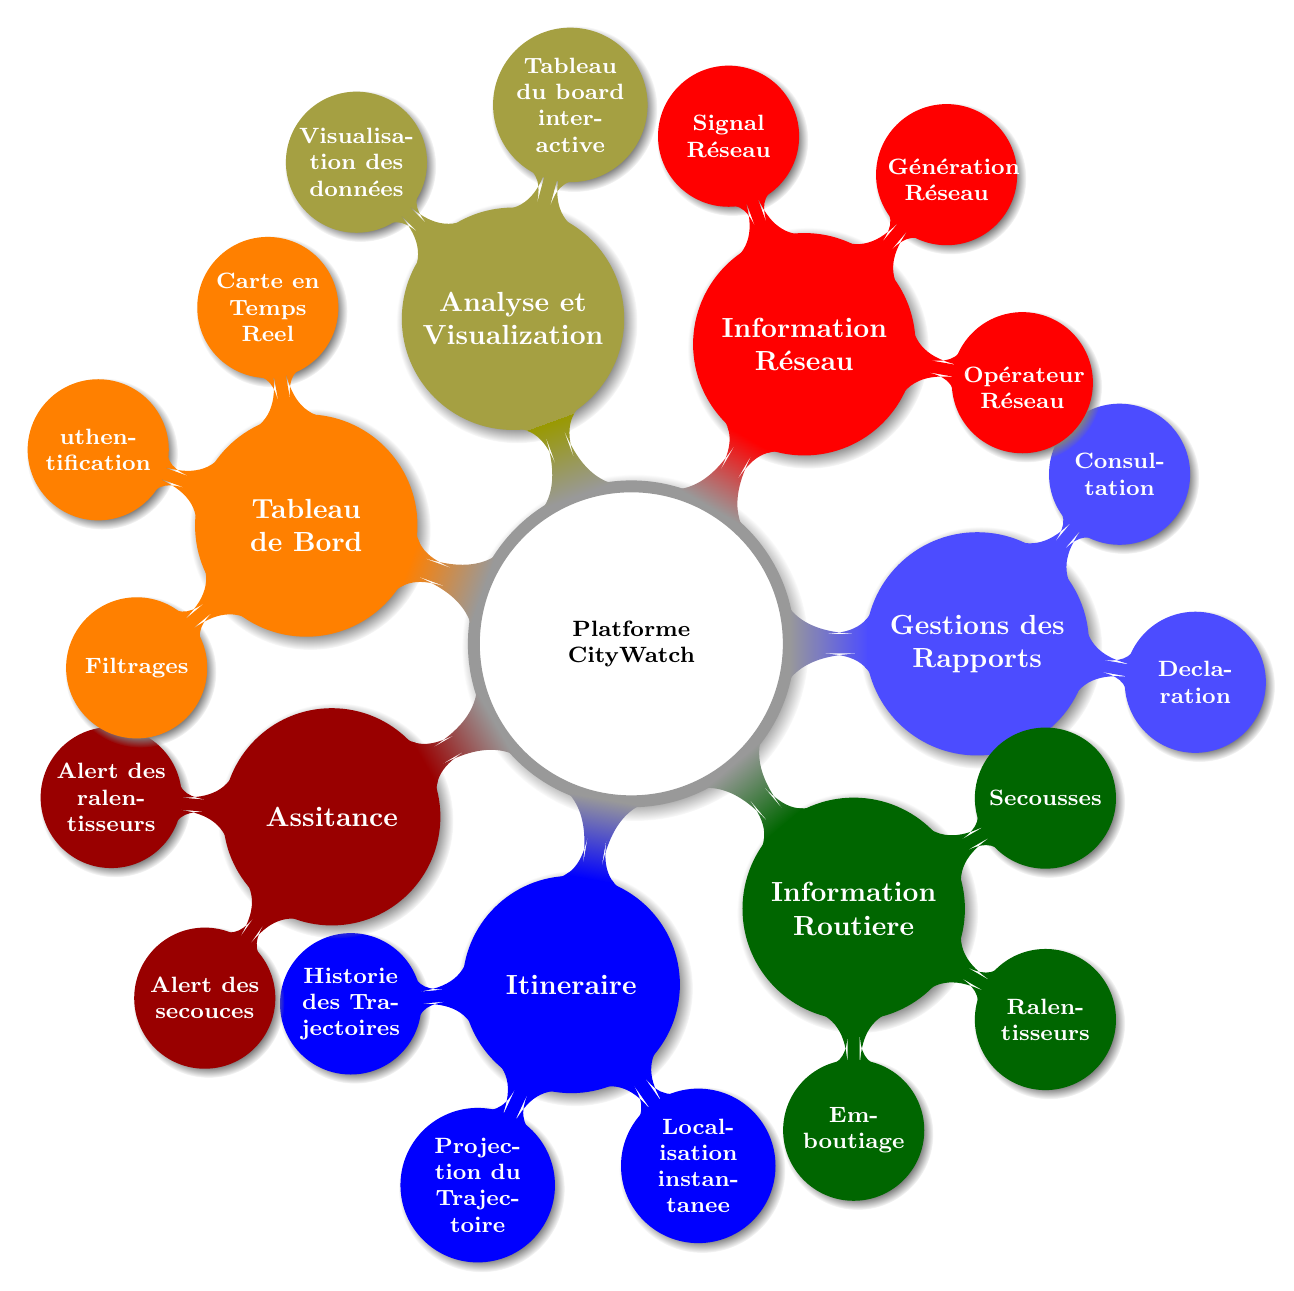
\begin{tikzpicture}[every annotation/.style={draw, fill=white, font=\Large}]
    \renewcommand{\href}[2]{#2}

    \path[mindmap,
          concept color=black!40,
          text=white,
          every node/.style={
              concept,
              circular drop shadow,
              execute at begin node=\hskip0pt,
          },
          %grow cyclic,
          root/.style={
              concept color=black!40,
              fill=white, line width=1ex, text=black,
              font=\footnotesize\bfseries,
              text width=7em},
          level 1 concept/.append style={
              font=\normalsize\bfseries,
              sibling angle=50,
              text width=7.7em,
              level distance=12.5em,
              inner sep=0pt},
          level 2 concept/.append style={
              font=\footnotesize\bfseries,
              level distance=8em},
          ours/.append style = {
              line width=0.5ex,
              concept color = black,
          }
    ]

    node[root] {Platforme CityWatch} [clockwise from=0]

    child[concept color=blue!70] {
        node {\ul{Gestions des Rapports}} [clockwise from=50]
        child { node { \ul{Consultation} } }
        child { node { \ul{Declaration} } }
    }
    child[concept color=green!40!black] {
        node[concept] {\ul{Information Routiere}} [clockwise from=30]
        child { node[concept] {\ul{Secousses}} }
        child { node[concept] {\ul{Ralentisseurs}}}
        child { node[concept] {Emboutiage}}
    }
    child[concept color=blue] {
        node[concept] {\ul{Itineraire}} [clockwise from=305]
        child { node[concept] {\ul{Localisation instantanee}} }
        child { node[concept] {\ul{Projection du Trajectoire}} }
        child { node[concept] {\ul{Historie des Trajectoires}} }
    }
    child[concept color=red!60!black] {
        node[concept] {Assitance} [clockwise from=235]
        child { node[concept] {Alert des secouces} }
        child { node[concept] {Alert des ralentisseurs} }
    }
    child[concept color=orange] {
        node[concept] {\ul{Tableau de Bord}} [counterclockwise from=100]
        child { node[concept] {\ul{Carte en Temps Reel}}}
        child { node[concept] {\ul{uthentification}} }
        child { node[concept] {\ul{Filtrages}} }
    }
    child[concept color=yellow!60!black] {
        node[concept] (Blogs) {\ul{Analyse et Visualization}} [clockwise from=135]
        child { node[concept] {Visualisation des données}}
        child { node[concept] {\ul{Tableau du board interactive}}}
    }
    child[concept color=red] {
        node[concept] {Information Réseau} [clockwise from=110]
        child { node[concept] {Signal Réseau} }
        child { node[concept] {Génération Réseau} }
        child { node[concept] {Opérateur Réseau} }
    };
    %\info{goForum.north east}{above,anchor=west,xshift=1em}{%
    %  \item[] Seit 2008
    %  \item 68\,444 Beiträge
    %  \item 13\,715 Themen
    %  \item 5\,532 registrierte Nutzer
    %}
    %\info{LaTeXForum.north west}{above,anchor=south}{%
    %  \item[] Seit 2008
    %  \item 81\,991 Beiträge
    %  \item 21\,026 Themen
    %  \item 13\,354 registrierte Nutzer
    %}
    %\info[8]{LaTeXArtikel.west}{below,anchor=north east,xshift=3em,yshift=-2em}{%
    %  \item 115 Artikel
    %}
    %\info[11]{LaTeXNews.south west}{below,anchor=north}{%
    %  \item 240 Meldungen
    %}
    %\info[9]{TikZGalerie.south}{below,anchor=north}{%
    %  \item[] Seit 2006
    %  \item 172 Autoren
    %  \item 384 Beispiele
    %}
    %\info[15]{goWiki.south}{below,anchor=north,xshift=3em}{%
    %  \item 152 erklärte Konzepte, Befehle und Pakete
    %}
    %\info{TeXweltQA.south east}{above,anchor=north west}{%
    %  \item[] Seit 2013
    %  \item 1\,710 Fragen
    %  \item 2\,151 Antworten
    %  \item 479 registrierte Nutzer
    %}
    %\info[8]{TeXweltBlog.south}{below,anchor=north,xshift=2em}{%
    %  \item[] Seit 2013
    %  \item 14 Autoren
    %}
    %\info[9]{PGFPlots.south west}{anchor=north east,xshift=1em}{%
    %  \item 14 Autoren
    %  \item 59 Beispiele
    %}
    %\info[6]{Planet.west}{anchor=east}{%
    %  \item 46 Blogs
    %}
    %\info[14]{TeXnique.east}{anchor=west,xshift = 0.5em}{%
    %  \item[] 2015, aufgrund Idee mit französischen
    %          \TeX-Freunden nach der TUG Damstadt, experimentell
    %}
    %\info[16]{Cookbook.east}{anchor=south west}{%
    %  \item[] Ab 10/2015, soll ca. 100 Beispiele aus
    %          dem \LaTeX\ Cookbook zeigen, sowie
    %          Community-Rezepte
    %}
\end{tikzpicture}
\caption{Objective du produit}
\label{fig:product-backlog}
\end{figure}
